%=== CHAPTER THREE (3) ===
%=== (Actual work done and contribution, including literature survey) ===

\chapter{Approach}

\section{CORBSLAM with Illumination Variance}

To enhance the ability of CORB-SLAM to map in different illumination conditions and seasons, Illumination Variance method is combined into the map fusion modules of CORB-SLAM server. The block diagram of the integrated system is illustrated in Figure \ref{fig:coislamoverview}.

\begin{figure}[H]
	\centering
	
\includegraphics[width=5in]{thereisafigure.eps}
	\caption{The block diagram of the modified system of CORB-SLAM integrated with illumination variance.}
	\label{fig:coislamoverview} 
\end{figure}

In the client end, the following modifications are made:

\begin{enumerate}
	\item A new thread running in parallel is added to process the input frame to transform into illumination variance images, and extract ORB keypoints in produced images (named as \textsl{II keypoints} in this paper).
	\item II keypoint data is added into each frame as new member variables. And then following the CORB-SLAM methodology, only the integrated keyframes are transmitted to the server,  which are serialized and packed by boost serialization library, and transmitted through ROS service.
\end{enumerate}

Besides the above changes, the following modification are made in the server end:

\begin{enumerate}
	\item A new keydataset containing II keypoint information. 
	\item A new illumination variance localizer running in parallel with the rgb localizer. When processing the input keyframe, a new localizer thread is started if the rgb localizer returns no result. The results from rgb and illumination variance localizer are currently added together in this work.
\end{enumerate}

\section{Quantitative Trajectory Evaluation Method}
To evaluate the mapping performance, the proposed method in \cite{zhang2018tutorial} is modified to multi robot case, and employed in this work.

The previous work of CORB-SLAM in \cite{li2017corb} only provides a rough overview of the mapping result of the multi robot system, as seen in Figure \ref{fig:corbslamresult}.

In \cite{maddern2014illumination} and \cite{arroyo2016openable}, the results of the illumination variance localization are also only briefly introduced, with no quantitative results given.

 In this paper, mapping results of CORB-SLAM and CORB-SLAM integrated with  is evaluated following the quantitative trajectory evaluation method proposed in \cite{zhang2018tutorial}.
 
\begin{figure}[H]
	\centering
	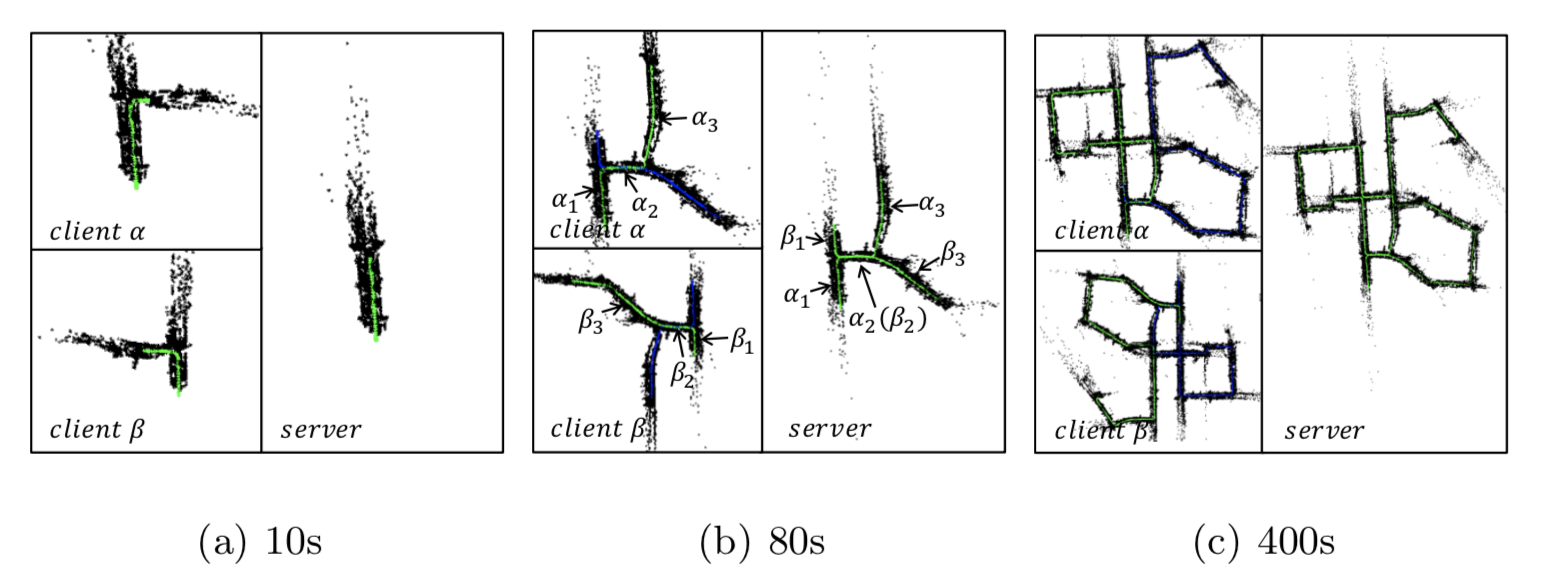
\includegraphics[width=5in]{Chapter3/corbslamresult.eps}
	\caption{Mapping results of CORB-SLAM in \cite{li2017corb}.}
	\label{fig:corbslamresult} 
\end{figure}



%=== END OF CHAPTER THREE ===
\newpage
